\documentclass[10pt]{beamer}
\usecolortheme{beetle}
\setbeamersize{text margin left=20pt,text margin right=20pt} 
%\setbeamertemplate{footline}[frame number]
\newcommand\mytext{some text}
\setbeamerfont{footline}{size=\fontsize{9}{11}\selectfont}
\setbeamercolor{section in toc}{fg=black}
\setbeamertemplate{footline} [text line]{%
	\parbox{\linewidth}{\vspace*{-20pt}\insertsection\hfill\textcolor{white}{\insertframenumber}\ / \inserttotalframenumber}
}
\setbeamertemplate{section in toc}[sections numbered]
\makeatletter
\setbeamertemplate{title page}{
  \vbox{}
  \vfill
  \begingroup
    \centering
    \begin{beamercolorbox}[sep=8pt,center]{title}
      \usebeamerfont{title}\inserttitle\par%
      \ifx\insertsubtitle\@empty%
      \else%
        \vskip0.25em%
        {\usebeamerfont{subtitle}\usebeamercolor[fg]{subtitle}\insertsubtitle\par}%
      \fi%     
    \end{beamercolorbox}%
    \vskip1em\par
    \begin{beamercolorbox}[sep=4pt,center]{author}
      \usebeamerfont{author}\insertauthor
    \end{beamercolorbox}
    \begin{beamercolorbox}[sep=8pt,center]{institute}
      \usebeamerfont{institute}\insertinstitute
    \end{beamercolorbox}
    % ----------------------- new
    \begin{beamercolorbox}[sep=4pt,center]{author}
      \usebeamerfont{author}presented by Ulla Aeschbacher
    \end{beamercolorbox}
    \begin{beamercolorbox}[sep=8pt,center]{institute}
      \usebeamerfont{institute} Institute of Computer Science, ETH Z\"urich
    \end{beamercolorbox}
    % ------------------------
    \begin{beamercolorbox}[sep=8pt,center]{date}
      \usebeamerfont{date}\insertdate
    \end{beamercolorbox}\vskip0.5em
    {\usebeamercolor[fg]{titlegraphic}\inserttitlegraphic\par}
  \endgroup
  \vfill
}
\makeatother

\beamertemplatenavigationsymbolsempty 								%suppress bar
\usepackage{tabularx}
\usepackage{tikz}
\usepackage{pgfplots}
\usetikzlibrary{calc,intersections,through,backgrounds, shapes}
\parindent=0cm

\newcommand{\bitem}{\begin{itemize}}									%begin{itemize}
\newcommand{\eitem}{\end{itemize}}										%end{itemize}

\tikzset{triangle/.style={regular polygon, regular polygon sides=3, draw, inner sep=0pt, minimum size=0.2cm}}
\tikzset{square/.style={regular polygon, regular polygon sides=4, draw, inner sep=0pt, minimum size=0.2cm}}
\tikzset{mydiamond/.style={diamond, draw, inner sep=0pt, minimum size=0.2cm}}
\tikzset{mycircle/.style={circle, draw, inner sep=0pt, minimum size=0.2cm}}

\definecolor{mred}{rgb}{0.82, 0.1, 0.26}
\definecolor{mblue}{rgb}{0.0, 0.3, 0.8}
\definecolor{mgreen}{rgb}{0.0, 0.8, 0.0}
\definecolor{mpink}{rgb}{0.8, 0.0, 0.6}

\definecolor{mgrey1}{rgb}{0.85, 0.85, 0.85} %lightest grey
\definecolor{mgrey2}{rgb}{0.7, 0.7, 0.7} 
\definecolor{mgrey3}{rgb}{0.3, 0.3, 0.3}
\definecolor{mgrey4}{rgb}{0.1, 0.1, 0.1} %darkest grey
\definecolor{background}{rgb}{0.6, 0.6, 0.6}

\begin{document}

\title {On Graphs, GPUs, and Blind Dating}
\subtitle{A Workload to Processor Matchmaking Quest}
\author[Gharaibeg, Costa, Santos-Neto, Ripeanu]{Abdullah Gharaibeh, Lauro Beltrão Costa, Elizeu Santos-Neto, Matei Ripeanu}
\institute{Department of Electrical and Computer Engineering\\The University of British Columbia}
\date{17.4.18}
\subject{Computer Science}
\frame{\titlepage}

%This paper wants to provide strategies on how to partition graphs and match those partitions to CPUs and GPUs. It gives a detailed evaluation of the performance impact of those strategies and explains the reasons for the observed performance in detail.
\section{Goal of Paper}
\frame{
\frametitle{Goal of Paper}
\bitem
	\item Explore effectiveness of graph partitioning strategies and workload allocation schemes to maximize performance
	\item Give evaluation of said performance
\eitem
}


\begin{frame}
\frametitle{Overview}
\tableofcontents
% First I will give a short summary of what the authors wanted to achieve
% Then I will give some necessary background and mention some related works
% Afterwards  I will give the characteristics of the workloads and the hybrid system that was used
% Next comes the most important part: the strategy how to partition the graph 
% Then comes the extensive evaluation to see if our strategy works
% Finally a short summary and some personal comments on the paper
\end{frame}


\section{Related Work and Background}
\frame{
\frametitle{Related Work}
%There is actually a triplet of papers from the same authors on this topic
 \bitem 
	 %In the first one they introduce the concept of processing graphs on heterogeneous platforms and introduce TOTEM, processing engine. I will go into further detail on TOTEM in a moment
 	\item September 2012: A Yoke of Oxen and a Thousand Chickens for Heavy Lifting Graph Processing 
	\pause
	% In the paper I am presenting today, they want to explore the effectiveness of three partitioning strategies and workload allocation schemes
	\item May 2013: \textcolor{white}{On Graphs, GPUs, and Blind Dating} 
	\pause
	%And in the third paper, they build on their previous work to try to answer the question on wether it is energy-efficient to partition the graph and use a hybrid system. the answer to this question is actually yes.
	\item November 2013: The Energy Case for Graph Processing on Hybrid CPU and GPU Systems
\eitem
}

%Now for a bit more background on the totem computation model
\frame{
\frametitle{\textsc{Totem} Computation Model}
\bitem
	%It divides processing into rounds, also called supersteps, and each round into phases.
	\item Processing divided into rounds 
	\item Rounds consisting of three phases
	\bitem
		\item Computation \\[0.3em]% In the first phase, each processing element (CPUs&GPUs) execute computations asynchronously on local memory
		\item Communication \\[0.3em]% The second phase consists of processors exchanging messages to update their status. This is the part where TOTEM shines, as it reduces communication overhead by aggregating  processor messages targeted to the same remote destination vertex at the source.
		\item Synchronization % This final phase guarantees delivery of messages. Specifically, a message sent at superstep i is guaranteed to be available in the local memory of the destination processor only at superstep i+1.
	\eitem
	%The whole reason behind using TOTEM is that because we reduce communication here, we can focus on reducing computation in the actual  graph partition strategy
\eitem
}

\iffalse
\frame{
\frametitle{Related Work}
\bitem
	\item Graph partitioning % lots of work, but normally focuses on partitioning a graph in a balanced way while minimizing the edge cut. we actually do not want a balanced partitioning, but instead partitions optimized for the two different processors
	\item Optimize graph algorithms on either GPU or CPU alone % some of which they mention could be applied to their BFS kernel to make it even faster
\eitem
}
\fi

%Now for the characteristics that define most real-world graph workloads, which they will be testing their strategy on for the most part.
\section{Characteristics}
\frame{
\frametitle{Characteristics of (Most) Real-World Graph Workloads}
\bitem
	%There is only modest processing per vertex per round.
	\item Modest processing per vertex per round 
	\pause
	%There is poor locality, so neighbors of a vertex are scattered in memory, 
	\item Poor locality 
	\pause
	%The graph displays a power-law degree distribution. This means that few vertices have many edges and most vertices have only a few edges. Graphs with this attribute are also called scale-free graphs.
	\item Power-law degree distribution\\[3em] 
	%\pause
	%For comparison we also test our strategy on graphs with a unform degree distributin, so that all vertices have an average number of edges.
	%\item Some tests on graphs with uniform degree distribution for comparison

\eitem
}

%A quick overview over the system the authors used to run their tests
\frame{
\frametitle{Characteristics of Hybrid System}
\begin{minipage}{0.5\textwidth}
%For the CPU, they used an Intel one from 2010 with 6 cores
\textcolor{white}{CPU} Intel Nehalem Xeon X5650
\bitem
	\item 2 $\times$ core frequency
	\item 24.6 $\times$ more memory
	\item 6 $\times$ more cache
	\item retailed at 999\$
	\item[$\to$] Can process large graphs
\eitem
\end{minipage}
\begin{minipage}{0.48\textwidth}
%For the GPU, they used a Nvidia one from 2011 with 14 cores.
\textcolor{white}{GPU} Nvidia Tesla C2075
\bitem
	\item 16 $\times$ more hardware threads
	\item 4.5 $\times$ faster memory access
	\item retailed at 599\$
	\item[]  \hfill
	\item[$\to$] Can process graphs in parallel
\eitem
%They display the classic attributes of CPUs and GPUs with the CPU being clocked at a higher frequency and having more memory and cache, while the GPU has more threads and faster memory access. The CPU is thus able to process larger graphs, while the GPU can process the (smaller) graphs in parallel.
\end{minipage}
}

%Now that we know the characteristics of our workloads and our hardware, we need to figure out how to best partition the graphs to fit the processors. There are some features that are required for any effective partitioning strategy
\section{Partitioning Strategy}
\frame{
\frametitle{Required Features for Graph Partitioning Strategies}
\bitem
	% The strategy needs to have low space and time complexitiy. Anything higher than linear is impractical
	\item Low space and time complexity 
	\pause
	% It has to handle scale-free graphs, which are, as mentioned, graphs where few vertices have many edges and most vertices have only a few edges
	\item Handles scale-free graphs
	\pause
	% The strategy has to be able to handle large graphs, up to half a billion vertices and eight billion edges
	\item Handles large graphs 
	\pause
	% It needs to reduce computation not communication, as the communication overhead is already minimized by using TOTEM model
	\item Reduces computation not communication 
\eitem
}

%Now we come to the actual partition strategy that the authors used 
\frame{
\frametitle{Partitioning Strategy}
%Their strategy is simple: Placing high-degree vertices in one type of processor \\ and low-degree ones in the other type.
 \center\textcolor{white}{Placing high-degree vertices in one type of processor \\ and low-degree ones in the other type.} \\[2em]
%There are mutliple reasons to justify this:
\bitem
	% The resulting partitions have different degrees of parallelism and thus suite the different processing elements of our hybrid system
	\item Partitions have different degrees of parallelism 
	%The partitions are within themselves more homogenous in terms of vertex connectivity which results in more balanced workload within a partition
	\item Partitions are more homogenous in terms of vertex connectivity 
	% We can do a partial sorting in linear time and in place, thus this strategy has low space and time complexity
	\item Low cost in terms of computational and space complexity 
\eitem
}

%One can apply this strategy in two different ways. 
\frame{
\frametitle{Three Different Partitioning Strategies}
\bitem
	% One can assign the highest-degree vertices to CPU and the lowest-degree vertices to GPU or vice-versa, called HIGH and LOW respectively.
	\item \textcolor{mgreen}{HIGH:} highest-degree vertices to CPU, lowest-degree vertices to GPU \\[2em]
	\item \textcolor{mred}{LOW:} lowest-degree vertices to CPU, highest-degree vertices to GPU \\[2em]
	% The authors also always run a random partitioning for comparison
	\item \textcolor{mblue}{RAND:} partitions the graph randomly
\eitem
}

%Now we come to the biggest part of the paper, the evaluation.
\section{Evaluation}
\frame{
\frametitle{Evaluation}
\bitem
	% The authors evaluate their strategy on two different example algorithms
	%First Breadth-First-Search, with an algorithm based on the the level-synchronous one by Hong et al. that we saw here last week. This algorithm is very sensitive to cache utilization.
	\item  \textcolor{white} {Breadth-First Search (BFS):} based on the level-synchronous one by Hong et al.\\[2em]
	%Second PageRank, an algorithm that ranks websites in Google Search by assigning weights to hyperlinks connecting them. This is a more compute intensive algorithm.
	\item  \textcolor{white} {PageRank:} algorithm used by Google Search to rank websites in their search engine results by assigning weights to hyperlinks
\eitem
}

%The authors show various different evaluations
\frame{
\frametitle{Evaluation}
\bitem
	%They show two different-sized scale-free graphs both for BFS and PageRank. scale-25 means that the graph has 2^25 vertices and 2^29 edges
	\item Scale-25 and scale-28 \textcolor{white}{power-law degree distribution} graphs\\[2em]	
	%They show two different-sized uniform degree graphs for BFS
	\item Scale-25 and scale-28 \textcolor{white}{uniform degree distribution} graphs\\[2em]
	%Now the authors also show how BFS and PageRank perform with different hardware configurations (up to four CPUs and 2 GPUs) and graph scales (from scale-25 to scale-29). I will leave those parts out because of the time limit. They do show though that their performance for BFS was competitive with other results at the time, yet with lower cost. 
	%Dont say what graph type they used here, I assume it is RMAT
	\item Scale-25 to scale-29 graphs \textcolor{white}{different hardware configurations} 	
\eitem
}

%Now its time for some graphs
%DISCLAIMER: I copied those graphs from the paper, so the numbers may not be 100% correct
%%%%%%%%%%%%%%%%%%%%%%%%%%%%%%%%%%%
%we can see that RAND and HiGH perform best when we divide the graph 50/50, so the load can be balanced completely between the two processing units. on both sides it drops as the CPU or GPU respectively become the bottleneck
%we can see that the partitioning strategy where we put the lowest-degree vertices in the CPU performs the best.we can explain this result thorugh the "visited"-bit-vector. this is the vector in which all the vertices that have been assigned a level are stored. in the LOW strategy, the large GPU partition is denser than those of the other two strategies, which leads to better localitly, which in turn leads to the "visited"-bit-vector to be small and fit into the GPU memory.
\frame{
\frametitle{Evaluation} 
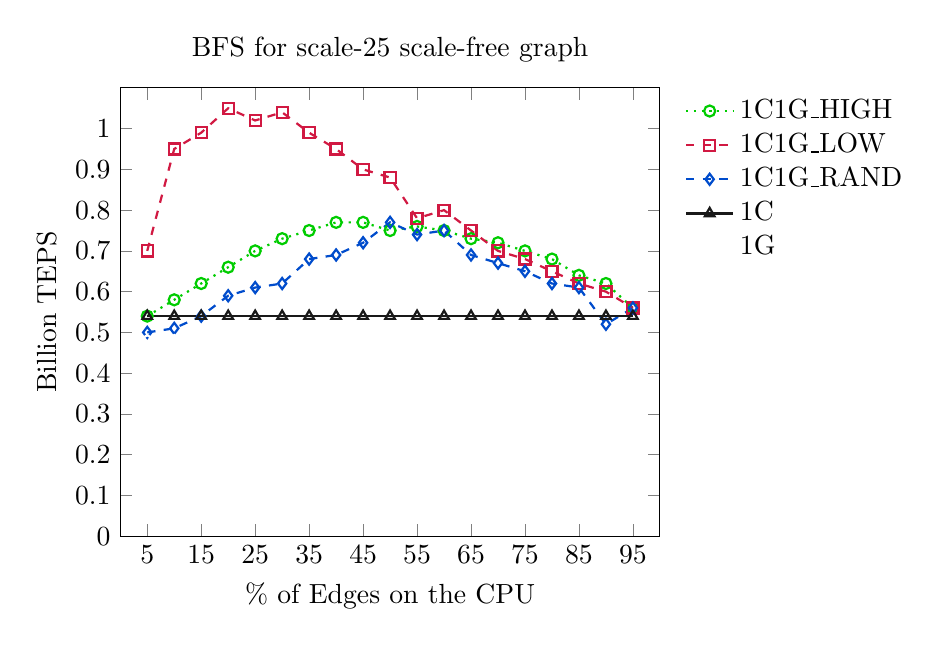
\begin{tikzpicture}
	\begin{axis}[
	title={BFS for scale-25 scale-free graph},
	xlabel={$\%$ of Edges on the CPU},
	ylabel={Billion TEPS},
	xmin=0, xmax=100,
	ymin=0.0, ymax=1.1,
	xtick={5,15,25,35,45,55,65,75,85,95},
	ytick={0,0.1,0.2,0.3,0.4,0.5,0.6,0.7,0.8,0.9,1.0},
	legend style={
		draw=none,
		fill=none, 
		legend pos=outer north east,
		cells={anchor=west},},
	]
	\addplot[
		color=mgreen,
		mark=o,
		mark options = {solid},
		dotted,
		thick] 
		coordinates {(5,0.54)(10,0.58)(15,0.62)(20,0.66)(25,0.7)(30,0.73)(35,0.75)(40,0.77)(45,0.77)(50,0.75)(55,0.76)(60,0.75)(65,0.73)(70,0.72)(75,0.7)(80,0.68)(85,0.64)(90,0.62)(95,0.56)};
	\addlegendentry{1C1G$\_$HIGH}
	\addplot[
		color=mred,
		mark=square,
		mark options = {solid},
		dashed,
		thick] 
		coordinates {(5,0.7)(10,0.95)(15,0.99)(20,1.05)(25,1.02)(30,1.04)(35,0.99)(40,0.95)(45,0.9)(50,0.88)(55,0.78)(60,0.8)(65,0.75)(70,0.70)(75,0.68)(80,0.65)(85,0.62)(90,0.6)(95,0.56)};
	\addlegendentry{1C1G$\_$LOW}
	\addplot[
		color=mblue,
		mark=diamond,
		mark options = {solid},
		dashed,
		thick] 
		coordinates {(5,0.5)(10,0.51)(15,0.54)(20,0.59)(25,0.61)(30,0.62)(35,0.68)(40,0.69)(45,0.72)(50,0.77)(55,0.74)(60,0.75)(65,0.69)(70,0.67)(75,0.65)(80,0.62)(85,0.61)(90,0.52)(95,0.56)};
	\addlegendentry{1C1G$\_$RAND}
	\addplot[
		color=mgrey4,
		mark=triangle,
		thick] 
		coordinates {(5,0.54)(10,0.54)(15,0.54)(20,0.54)(25,0.54)(30,0.54)(35,0.54)(40,0.54)(45,0.54)(50,0.54)(55,0.54)(60,0.54)(65,0.54)(70,0.54)(75,0.54)(80,0.54)(85,0.54)(90,0.54)(95,0.54)};
	\addlegendentry{1C}
	\addplot[
		color=white,
		mark=pentagon,
		thick] 
		coordinates {(5,0.48)(10,0.48)(15,0.48)(20,0.48)(25,0.48)(30,0.48)(35,0.48)(40,0.48)(45,0.48)(50,0.48)(55,0.48)(60,0.48)(65,0.48)(70,0.48)(75,0.48)(80,0.48)(85,0.48)(90,0.48)(95,0.48)};
	\addlegendentry{1G}
	\end{axis}
\end{tikzpicture}
}
%%%%%%%%%%%%%%%%%%%%%%%%%%%%%%%%%%%
%the CPU is here always the bottleneck, because the GPU can only hold a small partition of the graph. that is also why the graph begins at 70% of edges on the CPU.
%here we see that the HIGH strategy performs the best. this can be explained again through the size of the "visited"-bit-vector. With LOW and RAND, the CPU partition has a large number of vertices/edges and thus a large vector. due to the power-law degree distribution, the CPU partition produced by the HIGH strategy has much fewer vertices/edges and thus a smaller vector that is more cache friendly. the GPU can also handle the sparser part of the graph more efficiently.
\frame{
\frametitle{Evaluation}
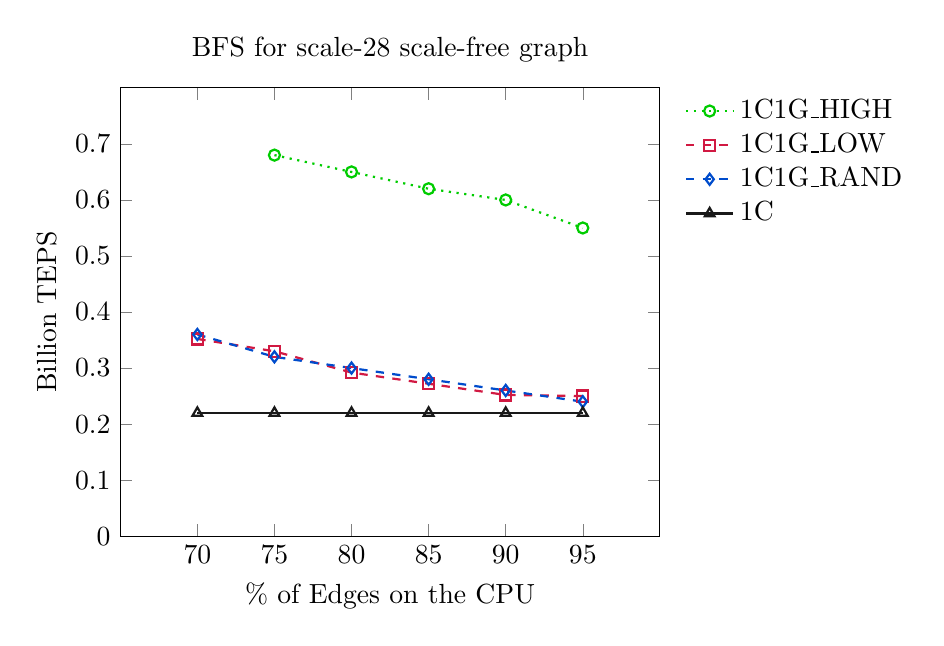
\begin{tikzpicture}
	\begin{axis}[
	title={BFS for scale-28 scale-free graph},
	xlabel={$\%$ of Edges on the CPU},
	ylabel={Billion TEPS},
	xmin=65, xmax=100,
	ymin=0.0, ymax=0.8,
	xtick={70,75,80,85,90,95},
	ytick={0,0.1,0.2,0.3,0.4,0.5,0.6,0.7},
	legend style={
		draw=none,
		fill=none, 
		legend pos=outer north east,
		cells={anchor=west},},
	]
	\addplot[
		color=mgreen,
		mark=o,
		mark options = {solid},
		dotted,
		thick] 
		coordinates {(75,0.68)(80,0.65)(85,0.62)(90,0.6)(95,0.55)};
	\addlegendentry{1C1G$\_$HIGH}
	\addplot[
		color=mred,
		mark=square,
		mark options = {solid},
		dashed,
		thick] 
		coordinates {(70,0.352)(75,0.33)(80,0.292)(85,0.272)(90,0.252)(95,0.25)};
	\addlegendentry{1C1G$\_$LOW}
	\addplot[
		color=mblue,
		mark=diamond,
		mark options = {solid},
		dashed,
		thick] 
		coordinates {(70,0.36)(75,0.32)(80,0.3)(85,0.28)(90,0.26)(95,0.24)};
	\addlegendentry{1C1G$\_$RAND}
	\addplot[
		color=mgrey4,
		mark=triangle,
		thick] 
		coordinates {(70,0.22)(75,0.22)(80,0.22)(85,0.22)(90,0.22)(95,0.22)};
	\addlegendentry{1C}
	\end{axis}
\end{tikzpicture}
}
%%%%%%%%%%%%%%%%%%%%%%%%%%%%
%because 1G is better than 1C, the peak is shifted to the left. 
%pagerank does more computation per vertex, placing few high-degree vertices on CPU allows processing them faster. 
\frame{
\frametitle{Evaluation} 
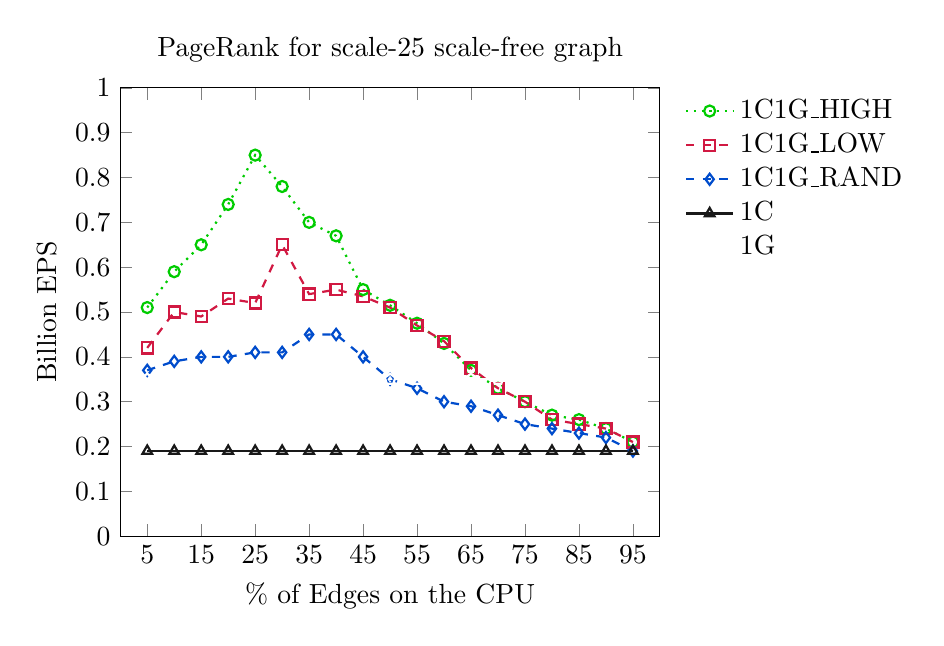
\begin{tikzpicture}
	\begin{axis}[
	title={PageRank for scale-25 scale-free graph},
	xlabel={$\%$ of Edges on the CPU},
	ylabel={Billion EPS},
	xmin=0, xmax=100,
	ymin=0.0, ymax=1.0,
	xtick={5,15,25,35,45,55,65,75,85,95},
	ytick={0,0.1,0.2,0.3,0.4,0.5,0.6,0.7,0.8,0.9,1.0},
	legend style={
		draw=none,
		fill=none, 
		legend pos=outer north east,
		cells={anchor=west},},
	]
	\addplot[
		color=mgreen,
		mark=o,
		mark options = {solid},
		dotted,
		thick] 
		coordinates {(5,0.51)(10,0.59)(15,0.65)(20,0.74)(25,0.85)(30,0.78)(35,0.7)(40,0.67)(45,0.55)(50,0.515)(55,0.475)(60,0.43)(65,0.37)(70,0.33)(75,0.30)(80,0.27)(85,0.26)(90,0.24)(95,0.21)};
	\addlegendentry{1C1G$\_$HIGH}
	\addplot[
		color=mred,
		mark=square,
		mark options = {solid},
		dashed,
		thick] 
		coordinates {(5,0.42)(10,0.50)(15,0.49)(20,0.53)(25,0.52)(30,0.65)(35,0.54)(40,0.55)(45,0.535)(50,0.51)(55,0.47)(60,0.435)(65,0.375)(70,0.33)(75,0.30)(80,0.26)(85,0.25)(90,0.24)(95,0.21)};
	\addlegendentry{1C1G$\_$LOW}
	\addplot[
		color=mblue,
		mark=diamond,
		mark options = {solid},
		dashed,
		thick] 
		coordinates {(5,0.37)(10,0.39)(15,0.4)(20,0.4)(25,0.41)(30,0.41)(35,0.45)(40,0.45)(45,0.4)(50,0.35)(55,0.33)(60,0.3)(65,0.29)(70,0.27)(75,0.25)(80,0.24)(85,0.23)(90,0.22)(95,0.19)};
	\addlegendentry{1C1G$\_$RAND}
	\addplot[
		color=mgrey4,
		mark=triangle,
		thick] 
		coordinates {(5,0.19)(10,0.19)(15,0.19)(20,0.19)(25,0.19)(30,0.19)(35,0.19)(40,0.19)(45,0.19)(50,0.19)(55,0.19)(60,0.19)(65,0.19)(70,0.19)(75,0.19)(80,0.19)(85,0.19)(90,0.19)(95,0.19)};
	\addlegendentry{1C}
	\addplot[
		color=white,
		mark=pentagon,
		thick] 
		coordinates {(5,0.35)(10,0.35)(15,0.35)(20,0.35)(25,0.35)(30,0.35)(35,0.35)(40,0.35)(45,0.35)(50,0.35)(55,0.35)(60,0.35)(65,0.35)(70,0.35)(75,0.35)(80,0.35)(85,0.35)(90,0.35)(95,0.35)};
	\addlegendentry{1G}
	\end{axis}
\end{tikzpicture}
}
%%%%%%%%%%%%%%%%%%%%%%%
%LOW partitioning allows for offloading a larger portion of the edges to the GPU, because with pageRank, the vertex itself uses more memory than in BFS. 
\frame{
\frametitle{Evaluation}
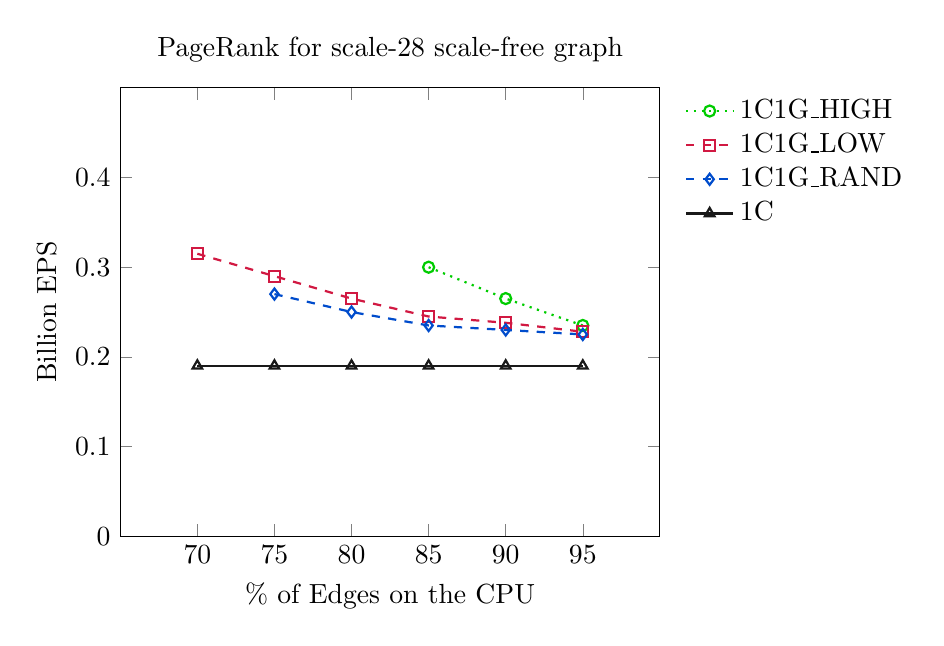
\begin{tikzpicture}
	\begin{axis}[
	title={PageRank for scale-28 scale-free graph},
	xlabel={$\%$ of Edges on the CPU},
	ylabel={Billion EPS},
	xmin=65, xmax=100,
	ymin=0.0, ymax=0.5,
	xtick={70,75,80,85,90,95},
	ytick={0,0.1,0.2,0.3,0.4},
	legend style={
		draw=none,
		fill=none, 
		legend pos=outer north east,
		cells={anchor=west},},
	]
	\addplot[
		color=mgreen,
		mark=o,
		mark options = {solid},
		dotted,
		thick] 
		coordinates {(85,0.3)(90,0.265)(95,0.235)};
	\addlegendentry{1C1G$\_$HIGH}
	\addplot[
		color=mred,
		mark=square,
		mark options = {solid},
		dashed,
		thick] 
		coordinates {(70,0.315)(75,0.29)(80,0.265)(85,0.245)(90,0.238)(95,0.228)};
	\addlegendentry{1C1G$\_$LOW}
	\addplot[
		color=mblue,
		mark=diamond,
		mark options = {solid},
		dashed,
		thick] 
		coordinates {(75,0.27)(80,0.25)(85,0.235)(90,0.23)(95,0.225)};
	\addlegendentry{1C1G$\_$RAND}
	\addplot[
		color=mgrey4,
		mark=triangle,
		thick] 
		coordinates {(70,0.19)(75,0.19)(80,0.19)(85,0.19)(90,0.19)(95,0.19)};
	\addlegendentry{1C}
	\end{axis}
\end{tikzpicture}
}
%%%%%%%%%%%%%%%%%%%%%%%%%%%%
% as you can see, the partition strategy does not matter here, as they all produce partitions with similar characteristics. Because GPU performs better, hybrid performance drops as CPU partition size increases. the best would be to put the whole thing on the GPU, because communication overhead would drop away. 
\frame{
\frametitle{Evaluation} 
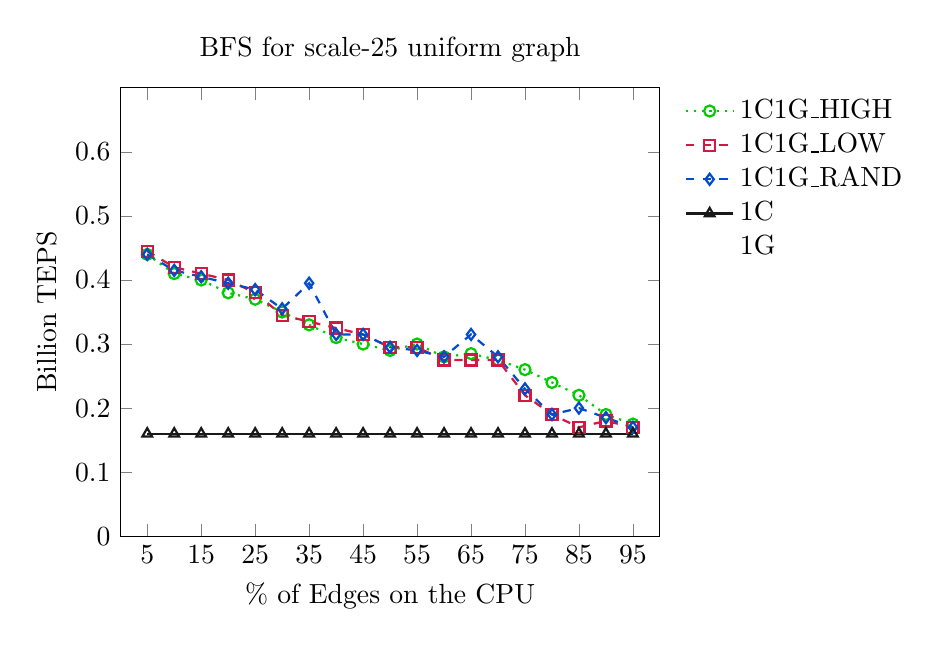
\begin{tikzpicture}
	\begin{axis}[
	title={BFS for scale-25 uniform graph},
	xlabel={$\%$ of Edges on the CPU},
	ylabel={Billion TEPS},
	xmin=0, xmax=100,
	ymin=0.0, ymax=0.7,
	xtick={5,15,25,35,45,55,65,75,85,95},
	ytick={0,0.1,0.2,0.3,0.4,0.5,0.6},
	legend style={
		draw=none,
		fill=none, 
		legend pos=outer north east,
		cells={anchor=west},},
	]
	\addplot[
		color=mgreen,
		mark=o,
		mark options = {solid},
		dotted,
		thick] 
		coordinates {(5,0.44)(10,0.41)(15,0.4)(20,0.38)(25,0.37)(30,0.35)(35,0.33)(40,0.31)(45,0.30)(50,0.29)(55,0.30)(60,0.28)(65,0.285)(70,0.275)(75,0.26)(80,0.24)(85,0.22)(90,0.19)(95,0.175)};
	\addlegendentry{1C1G$\_$HIGH}
	\addplot[
		color=mred,
		mark=square,
		mark options = {solid},
		dashed,
		thick] 
		coordinates {(5,0.445)(10,0.42)(15,0.41)(20,0.4)(25,0.38)(30,0.345)(35,0.335)(40,0.325)(45,0.315)(50,0.295)(55,0.295)(60,0.275)(65,0.275)(70,0.275)(75,0.22)(80,0.19)(85,0.17)(90,0.18)(95,0.17)};
	\addlegendentry{1C1G$\_$LOW}
	\addplot[
		color=mblue,
		mark=diamond,
		mark options = {solid},
		dashed,
		thick] 
		coordinates {(5,0.44)(10,0.415)(15,0.405)(20,0.395)(25,0.385)(30,0.355)(35,0.395)(40,0.315)(45,0.315)(50,0.295)(55,0.29)(60,0.28)(65,0.315)(70,0.28)(75,0.23)(80,0.19)(85,0.20)(90,0.185)(95,0.17)};
	\addlegendentry{1C1G$\_$RAND}
	\addplot[
		color=mgrey4,
		mark=triangle,
		thick] 
		coordinates {(5,0.16)(10,0.16)(15,0.16)(20,0.16)(25,0.16)(30,0.16)(35,0.16)(40,0.16)(45,0.16)(50,0.16)(55,0.16)(60,0.16)(65,0.16)(70,0.16)(75,0.16)(80,0.16)(85,0.16)(90,0.16)(95,0.16)};
	\addlegendentry{1C}
	\addplot[
		color=white,
		mark=pentagon,
		thick] 
		coordinates {(5,0.58)(10,0.58)(15,0.58)(20,0.58)(25,0.58)(30,0.58)(35,0.58)(40,0.58)(45,0.58)(50,0.58)(55,0.58)(60,0.58)(65,0.58)(70,0.58)(75,0.58)(80,0.58)(85,0.58)(90,0.58)(95,0.58)};
	\addlegendentry{1G}
	\end{axis}
\end{tikzpicture}
}
%%%%%%%%%%%%%%%%%%%%%%%%%
%when doing the same on a scale-28 uniform graph, we get a very interesting graph :) Here we do not gain anything from processing part of the graph on the GPU, because communication overhead masks the gain in reducing computation time.
\frame{
\frametitle{Evaluation} 
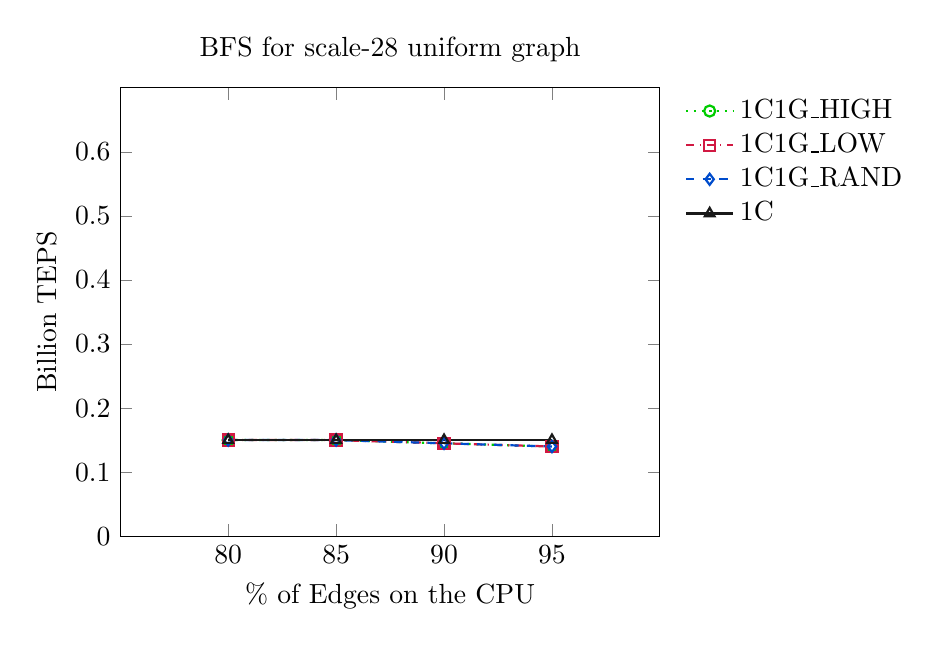
\begin{tikzpicture}
	\begin{axis}[
	title={BFS for scale-28 uniform graph},
	xlabel={$\%$ of Edges on the CPU},
	ylabel={Billion TEPS},
	xmin=75, xmax=100,
	ymin=0.0, ymax=0.7,
	xtick={80,85,90,95},
	ytick={0,0.1,0.2,0.3,0.4,0.5,0.6},
	legend style={
		draw=none,
		fill=none, 
		legend pos=outer north east,
		cells={anchor=west},},
	]
	\addplot[
		color=mgreen,
		mark=o,
		mark options = {solid},
		dotted,
		thick] 
		coordinates {(80,0.15)(85,0.15)(90,0.145)(95,0.14)};
	\addlegendentry{1C1G$\_$HIGH}
	\addplot[
		color=mred,
		mark=square,
		mark options = {solid},
		dash dot,
		thick] 
		coordinates {(80,0.15)(85,0.15)(90,0.145)(95,0.14)};
		\addlegendentry{1C1G$\_$LOW}
	\addplot[
		color=mblue,
		mark=diamond,
		mark options = {solid},
		dashed,
		thick] 
		coordinates {(80,0.15)(85,0.15)(90,0.145)(95,0.14)};
	\addlegendentry{1C1G$\_$RAND}
	\addplot[
		color=mgrey4,
		mark=triangle,
		thick] 
		coordinates {(80,0.15)(85,0.15)(90,0.15)(95,0.15)};
		\addlegendentry{1C}
	\end{axis}
\end{tikzpicture}
}

\frame{
\frametitle{Evaluation} 
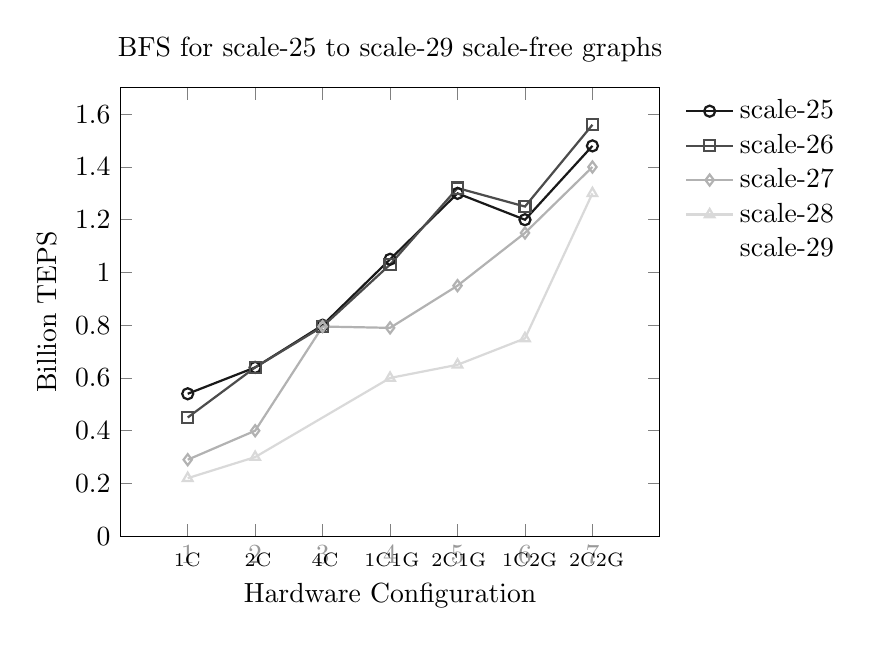
\begin{tikzpicture}
	\begin{axis}[
	title={BFS for scale-25 to scale-29 scale-free graphs},
	xlabel={Hardware Configuration},
	ylabel={Billion TEPS},
	xmin=0, xmax=8,
	ymin=0.0, ymax=1.7,
	xtick={1,2,3,4,5,6,7},
	ytick={0,0.2,0.4,0.6, 0.8, 1.0, 1.2, 1.4, 1.6},
	x tick label style={color=background},
	legend style={
		draw=none,
		fill=none, 
		legend pos=outer north east,
		cells={anchor=west},},
	]
	\addplot[
		color=mgrey4,
		mark=o,
		thick] 
		coordinates {(1,0.54)(2,0.64)(3,0.8)(4,1.05)(5,1.3)(6,1.2)(7,1.48)};
	\addlegendentry{scale-25}
	\addplot[
		color=mgrey3,
		mark=square,
		thick] 
		coordinates{(1,0.45)(2,0.64)(3,0.795)(4,1.03)(5,1.32)(6,1.25)(7,1.56)};
	\addlegendentry{scale-26}
	\addplot[
		color=mgrey2,
		mark=diamond,
		thick] 
		coordinates {(1,0.29)(2,0.4)(3,0.795)(4,0.79)(5,0.95)(6,1.15)(7,1.40)};
	\addlegendentry{scale-27}
	\addplot[
		color=mgrey1,
		mark=triangle,
		thick] 
		coordinates {(1,0.22)(2,0.30)(4,0.6)(5,0.65)(6,0.75)(7,1.3)};
	\addlegendentry{scale-28}
	\addplot[
		color=white,
		mark=pentagon,
		thick] 
		coordinates {(1,0.09)(2,0.1)(4,0.1)(5,0.11)(6,0.15)(7,0.19)};
	\addlegendentry{scale-29}
	\end{axis}
	\node at (0.85,-0.3) {\scriptsize1C};
	\node at (1.75,-0.3) {\scriptsize2C};
	\node at (2.6,-0.3) {\scriptsize4C};
	\node at (3.45,-0.3) {\scriptsize1C1G};
	\node at (4.3,-0.3) {\scriptsize2C1G};
	\node at (5.2,-0.3) {\scriptsize1C2G};
	\node at (6.05,-0.3) {\scriptsize2C2G};
\end{tikzpicture}
}

\frame{
\frametitle{Evaluation} 
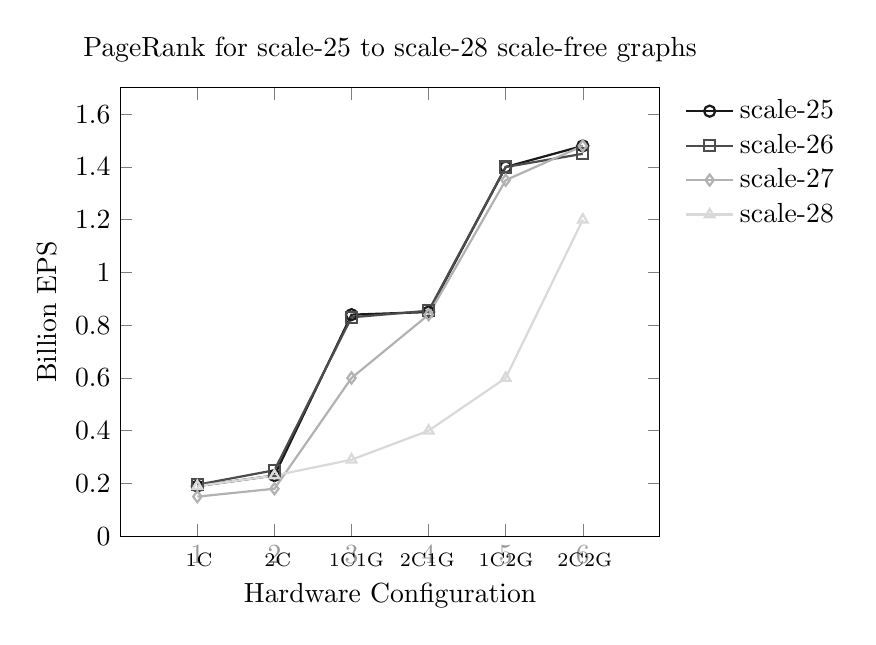
\begin{tikzpicture}
	\begin{axis}[
	title={PageRank for scale-25 to scale-28 scale-free graphs},
	xlabel={Hardware Configuration},
	ylabel={Billion EPS},
	xmin=0, xmax=7,
	ymin=0.0, ymax=1.7,
	xtick={1,2,3,4,5,6},
	ytick={0,0.2,0.4,0.6, 0.8, 1.0, 1.2, 1.4, 1.6},
	x tick label style={color=background},
	legend style={
		draw=none,
		fill=none, 
		legend pos=outer north east,
		cells={anchor=west},},
	]
	\addplot[
		color=mgrey4,
		mark=o,
		thick] 
		coordinates {(1,0.19)(2,0.23)(3,0.84)(4,0.85)(5,1.4)(6,1.48)};
	\addlegendentry{scale-25}
	\addplot[
		color=mgrey3,
		mark=square,
		thick] 
		coordinates {(1,0.195)(2,0.25)(3,0.83)(4,0.855)(5,1.4)(6,1.45)};
	\addlegendentry{scale-26}
	\addplot[
		color=mgrey2,
		mark=diamond,
		thick] 
		coordinates {(1,0.15)(2,0.18)(3,0.6)(4,0.84)(5,1.35)(6,1.48)};
	\addlegendentry{scale-27}
	\addplot[
		color=mgrey1,
		mark=triangle,
		thick] 
		coordinates {(1,0.19)(2,0.23)(3,0.29)(4,0.4)(5,0.6)(6,1.2)};
	\addlegendentry{scale-28}
	\end{axis}
	\node at (1,-0.3) {\scriptsize1C};
	\node at (2,-0.3) {\scriptsize2C};
	\node at (3, -0.3) {\scriptsize1C1G};
	\node at (3.9,-0.3) {\scriptsize2C1G};
	\node at (4.9,-0.3) {\scriptsize1C2G};
	\node at (5.9,-0.3) {\scriptsize2C2G};
\end{tikzpicture}
}

%After all those graphs I will try to put the results together into a short summary
\section{Summary}
\frame{
\frametitle{Summary}
\bitem
	%For BFS, we should use the HIGH partition strategy for large graphs, where only small fraction can fit into the GPU memory
	% and the LOW strategy for small graphs that fit mostly into the GPU memory
	\item Cache-sensitive algorithms:
	\bitem
		\item Large graphs: \textcolor{mgreen}{HIGH} 
		\item Small graphs: \textcolor{mred}{LOW} 
	\eitem
	%For PageRank it is vice-versa, because of the way memory is used
	\item More compute-intensive algorithms:
	\bitem
		\item Large graphs: \textcolor{mred}{LOW}
		\item Small graphs:  \textcolor{mgreen}{HIGH}
	\eitem
	%All in all hybrid systems do make sense, as they almost always out-perform non-hybrid systems
	\item Hybrid-system makes sense
	%This is only for scale-free graphs though, for uniform degree graphs it doesnt help at all
	\item Graph topology is important
\eitem
}

%My own opinion on this paper is generally a good one.
\frame{
\frametitle{Personal Review}
\bitem
	%They show that with simple strategies they can gain siginificant performance increase
	\item Simple partition strategy
	%They also show in great detail how much those strategies improve performance and give reasons as to why
	\item Show in great detail how it improves performance
	%They focus heavily on BFS, PageRank comes across more as a sidenote, even though it shows that the algorithm matters
	\item Focus is on BFS
	%Also the code is available, I have to admit though that I did not rerun the experiments myself.
	\item Code is available
	%All in all I did not find any irregularities in their arguments.
\eitem
}

%With that my presentation is finished and I will gladly answer your questions.
\frame{
\Huge{\textcolor{white}{Questions?}}
}






\end{document}
